\PassOptionsToPackage{quiet}{fontspec}
\documentclass[10pt,aspectratio=169]{beamer}
\usepackage{zju_beamer}
\usepackage{booktabs}
\usepackage{multirow}
\usepackage{amsmath}
\graphicspath{{./figures/}}
\zjusectioncolor{blue}
\setbeamertemplate{headline}{}
\setbeamertemplate{caption}[numbered]

\title[SE Growth Model]{Dynamic Predictive Model for Growth of \textit{Salmonella} Enteritidis in Egg Yolk}
\subtitle{Gompertz Model with Modified Ratkowsky Secondary Model}
\author[Group X]{Boyuan Zhao, Wenyu Xu, Yizhou Li}
\institute[ZJU]{College of Biosystems Engineering and Food Science \\ Zhejiang University}
\date{April 21, 2026}

\begin{document}

% ==================== Slide 1: Title ====================
\begin{frame}
\titlepage
\end{frame}

% ==================== Slide 2: Outline ====================
\section*{}
\begin{frame}{Outline}
\tableofcontents
\end{frame}

% ==================== Slide 3: Introduction ====================
\section{Introduction}
\begin{frame}{Introduction \& Background}
\begin{columns}[T]
\begin{column}{0.62\textwidth}
\begin{itemize}
    \item \textit{Salmonella} Enteritidis (SE) --- leading cause of foodborne illness
    \item Shell eggs: SE penetrates shell $\rightarrow$ grows in iron-rich yolk
    \item USDA-FSIS: eggs stored $\leq 7.2\,^\circ$C within 12\,h of laying
    \item Temperature fluctuates during cooling, storage, distribution
    \item \textbf{Objective:} Develop a dynamic Gompertz model for SE growth under sinusoidal temperature (3--43\,$^\circ$C)
\end{itemize}
\vspace{0.5em}
{\small Ref: Gumudavelli et al.\ (2007), \textit{J.\ Food Sci.}\ 72:M254--62}
\end{column}
\begin{column}{0.35\textwidth}
\centering
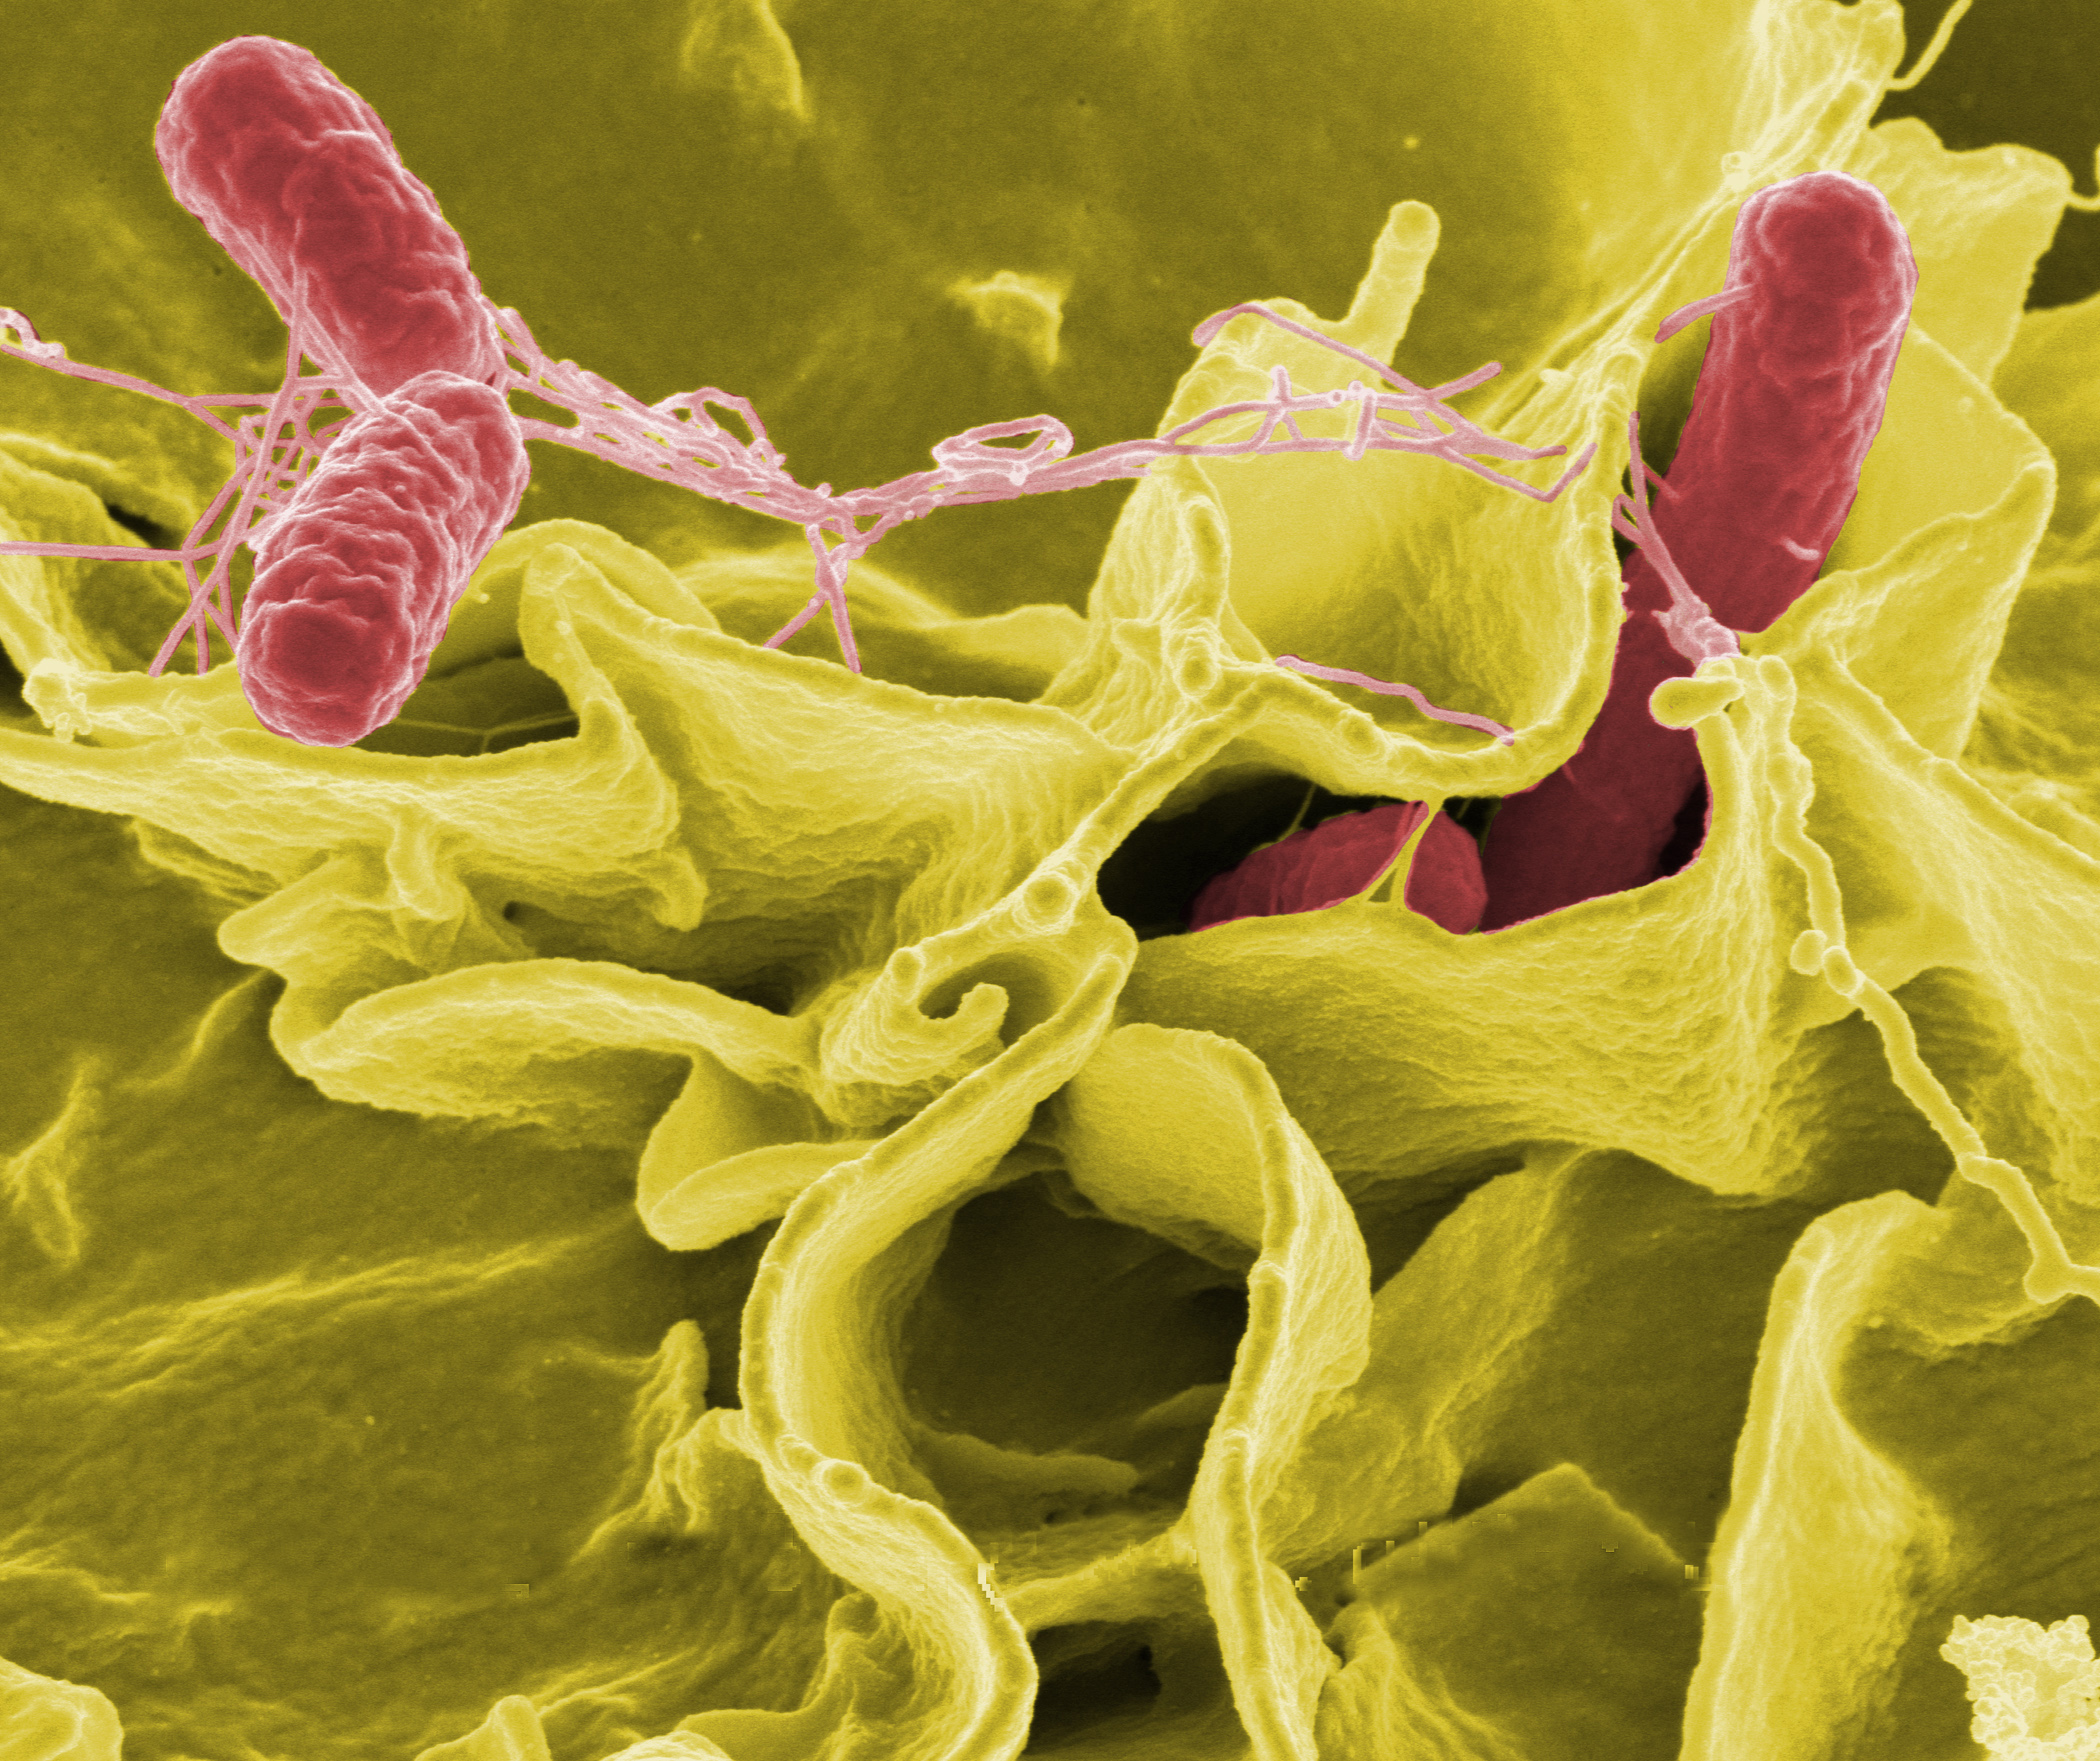
\includegraphics[width=0.85\linewidth]{salmonella_cdc.jpg}

{\scriptsize\textit{Salmonella} bacteria (colorized SEM).\\Source: NIAID/CDC, public domain.}
\end{column}
\end{columns}
\end{frame}

% ==================== Slide 4: Model ====================
\section{Model}
\begin{frame}{Model Description}
\begin{columns}[T]
\begin{column}{0.48\textwidth}
\textbf{Primary Model (Gompertz)}

Constant $T$ (analytical):
\begin{equation*}
y(t) = A + C \cdot e^{-e^{(\mu e / C)(M-t)+1}}
\end{equation*}

Variable $T$ (ODE):
\begin{equation*}
\frac{dy}{dt} = -\mu(T)\, e\, \frac{y-A}{C}\, \ln\!\left(\frac{y-A}{C}\right)
\end{equation*}

$y = \log_{10}N$;\; $A$: initial;\; $C$: range;\; $M$: inflection time
\end{column}
\begin{column}{0.48\textwidth}
\textbf{Secondary Model (Ratkowsky)}
\begin{equation*}
\mu(T) = a(T - T_{\min})^2 \left(1 - e^{b(T - T_{\max})}\right)
\end{equation*}

$a, b$: regression coefficients\\
$T_{\min} = 6\,^\circ$C,\; $T_{\max} = 46.3\,^\circ$C (fixed)

\vspace{1em}
\textbf{Dynamic Model}\\
Integrate primary + secondary,\\
solve numerically with \texttt{ode45}.\\
Temperature interpolated via \texttt{interp1}.
\end{column}
\end{columns}
\end{frame}

% ==================== Slide 5: Data & Parameters ====================
\section{Data \& Parameters}
\begin{frame}{Data \& Parameters}
\begin{columns}[T]
\begin{column}{0.45\textwidth}
\textbf{Data Summary}
\begin{itemize}
    \item Growth: 12 time points (0--17\,hr), 20 observations
    \item 0--2\,hr: single; 3--17\,hr: duplicates
    \item Temperature: 47 points, sinusoidal $\sim$7--43\,$^\circ$C
    \item Interpolated via \texttt{interp1}
\end{itemize}
\end{column}
\begin{column}{0.52\textwidth}
\centering
{\small
\begin{tabular}{llcc}
\toprule
Param & Description & Guess & Status \\
\midrule
$A$        & Init.\ $\log_{10}$(CFU/mL) & 2.60     & Est.\ \\
$C$        & Growth range               & 11       & Est.\ \\
$M$        & Inflection time (hr)       & 7.5      & Est.\ \\
$a$        & Ratkowsky coeff            & 3.38e-4  & Est.\ \\
$b$        & Ratkowsky coeff            & 0.275    & Est.\ \\
$T_{\min}$ & Min growth temp            & 6.0\,$^\circ$C  & Fixed \\
$T_{\max}$ & Max growth temp            & 46.3\,$^\circ$C & Fixed \\
\bottomrule
\end{tabular}}

\vspace{0.3em}
{\scriptsize Table 1. Model parameters and initial guesses.}
\end{column}
\end{columns}
\end{frame}

% ==================== Slide 6: Forward & SSC ====================
\section{Forward Problem}
\begin{frame}{Forward Problem \& Scaled Sensitivity Coefficients}
\begin{columns}[T]
\begin{column}{0.48\textwidth}
\centering
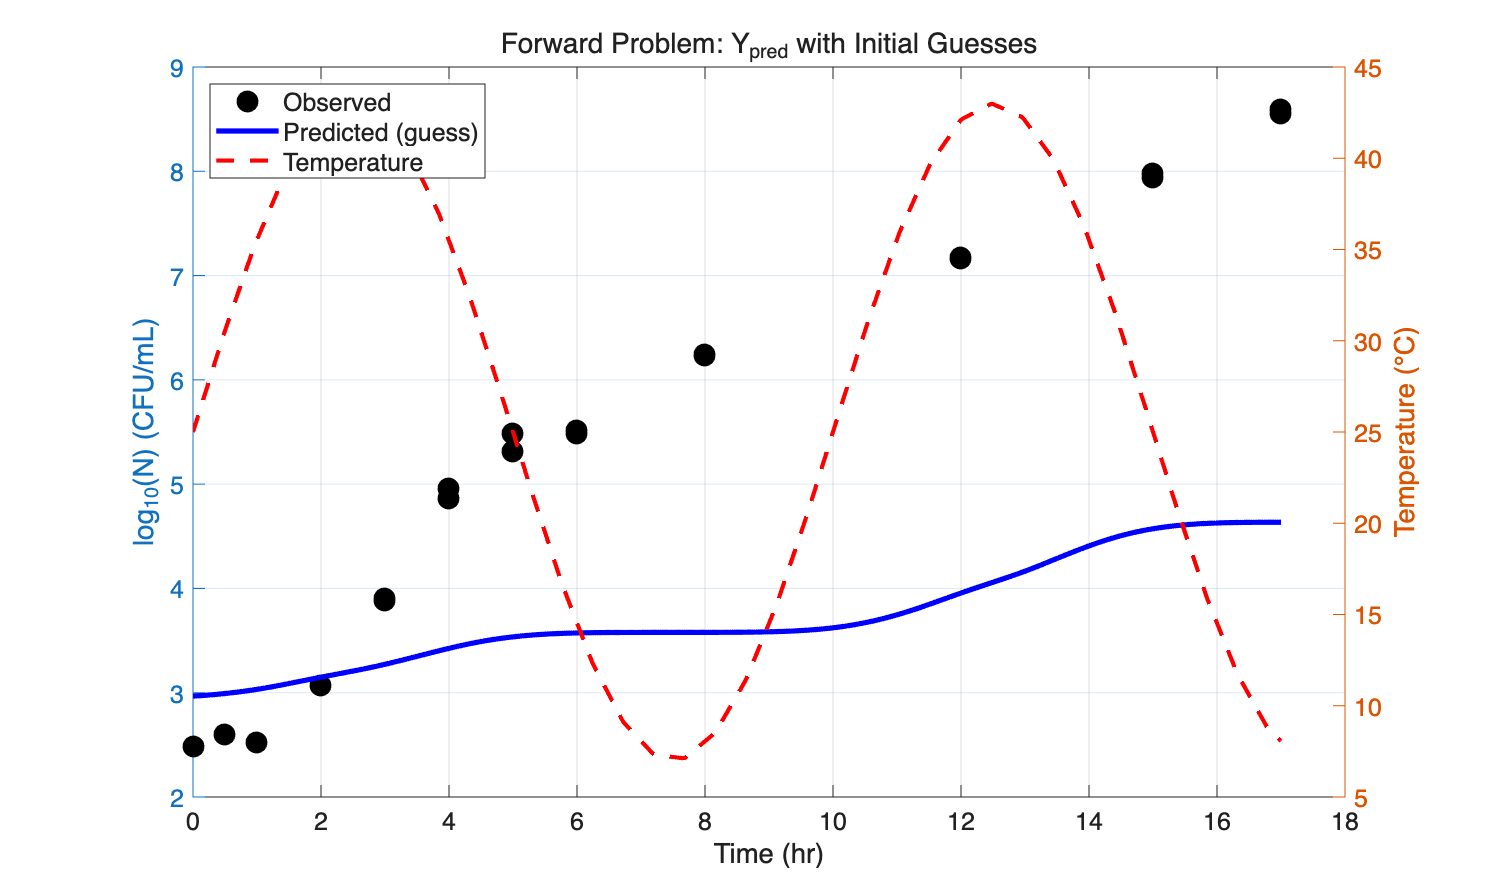
\includegraphics[width=\linewidth]{fig01_forward_guess.png}

{\scriptsize Fig.\,1. Forward prediction with initial guesses.\\Black: observed; Blue: predicted; Red: temperature.}
\end{column}
\begin{column}{0.48\textwidth}
\centering
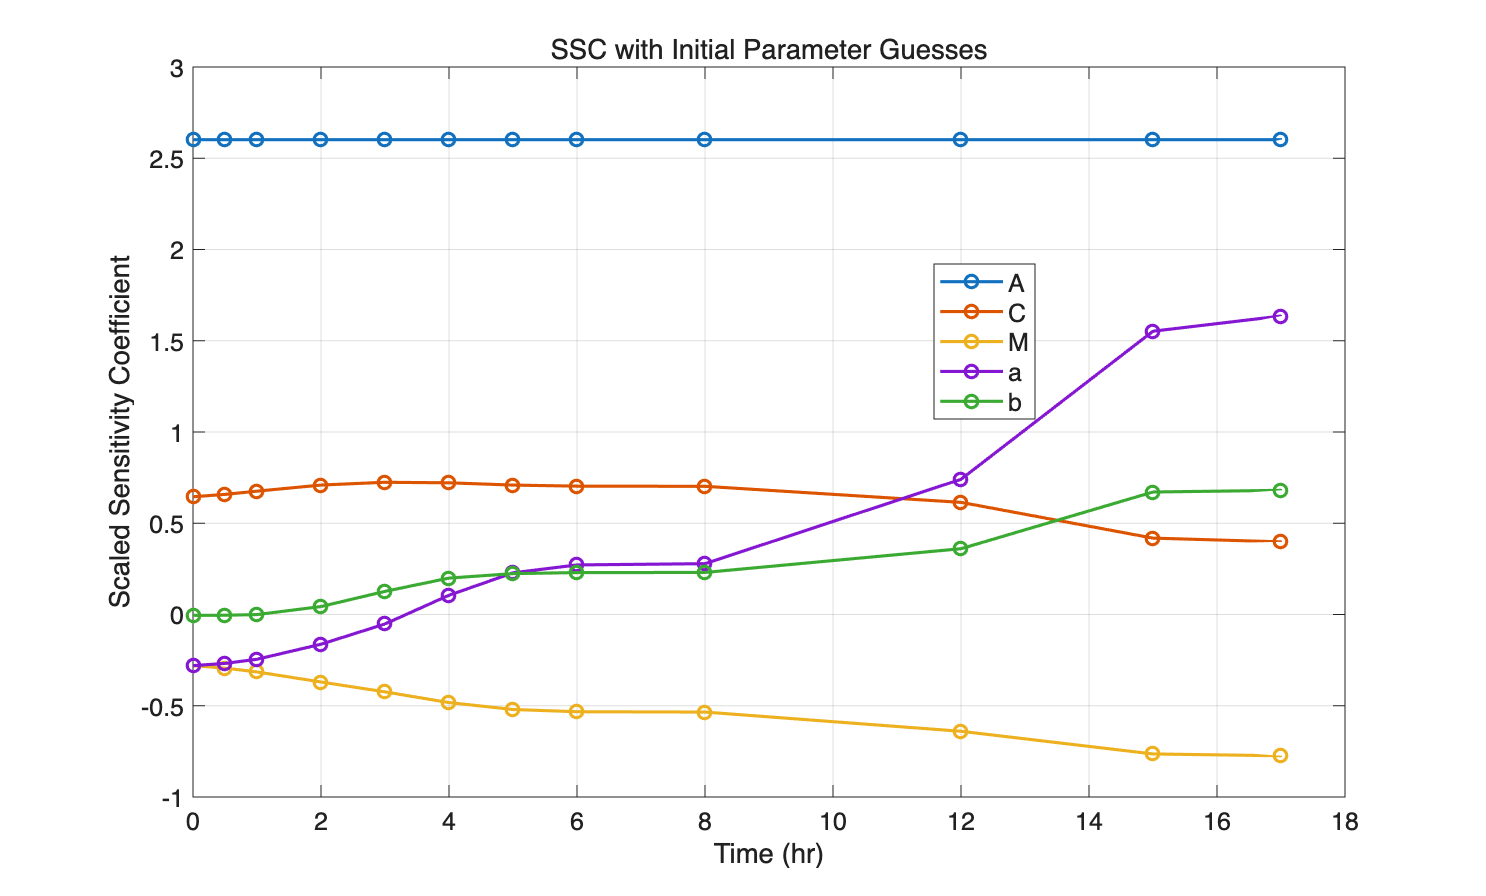
\includegraphics[width=\linewidth]{fig02_ssc_initial.png}

{\scriptsize Fig.\,2. Scaled sensitivity coefficients (SSC) at initial guesses. All 5 parameters show distinct patterns.}
\end{column}
\end{columns}
\vspace{0.3em}
{\small $T_{\min}$, $T_{\max}$ have negligible SSC $\rightarrow$ fixed at literature values.}
\end{frame}

% ==================== Slide 7: OLS Results ====================
\section{OLS Estimation}
\begin{frame}{OLS Parameter Estimates}
\centering
{\small
\begin{tabular}{lrrrrr}
\toprule
Param & Estimate & SE & Rel.Err (\%) & CI$_{\text{lo}}$ & CI$_{\text{hi}}$ \\
\midrule
$A$ & 2.4011 & 0.2540 & 10.58 & 1.8597 & 2.9425 \\
$C$ & 6.3798 & 0.4565 &  7.16 & 5.4067 & 7.3528 \\
$M$ & 2.9213 & 1.8074 & 61.87 & $-$0.9310 & 6.7736 \\
$a$ & 0.001135 & 0.000263 & 23.15 & 0.000575 & 0.001695 \\
$b$ & 0.2621 & 0.2180 & 83.20 & $-$0.2027 & 0.7268 \\
\bottomrule
\end{tabular}}

{\scriptsize Table 2. OLS parameter estimates with standard errors and 95\% confidence intervals.}

\vspace{0.8em}
{\small RMSE = 0.2524 $\log_{10}$ CFU/mL \hspace{2em} Pseudo-$R^2$ = 0.9874 \hspace{2em} MSE = 0.0637 \hspace{2em} $N$ = 20}
\end{frame}

% ==================== Slide 7b: Correlation ====================
\begin{frame}{Correlation Matrix}
\centering
{\small
\begin{tabular}{lccccc}
\toprule
      & $A$ & $C$ & $M$ & $a$ & $b$ \\
\midrule
$A$ &  1.000 & $-$0.834 &  0.808 & $-$0.281 &  0.459 \\
$C$ & $-$0.834 &  1.000 & $-$0.711 &  0.050 & $-$0.312 \\
$M$ &  0.808 & $-$0.711 &  1.000 & $-$0.601 &  0.826 \\
$a$ & $-$0.281 &  0.050 & $-$0.601 &  1.000 & $-$0.930 \\
$b$ &  0.459 & $-$0.312 &  0.826 & $-$0.930 &  1.000 \\
\bottomrule
\end{tabular}}

{\scriptsize Table 3. Parameter correlation matrix.}

\vspace{1em}
\begin{itemize}
    \item Strong correlation between $a$ and $b$ ($-$0.930) --- expected for Ratkowsky coefficients
    \item $M$ and $b$ also correlated (0.826) --- lag time linked to temperature sensitivity
    \item High correlations may increase parameter uncertainty but do not prevent estimation
\end{itemize}
\end{frame}

% ==================== Slide 8: CB & PB ====================
\begin{frame}{Fitted Curve with Confidence \& Prediction Bands}
\centering
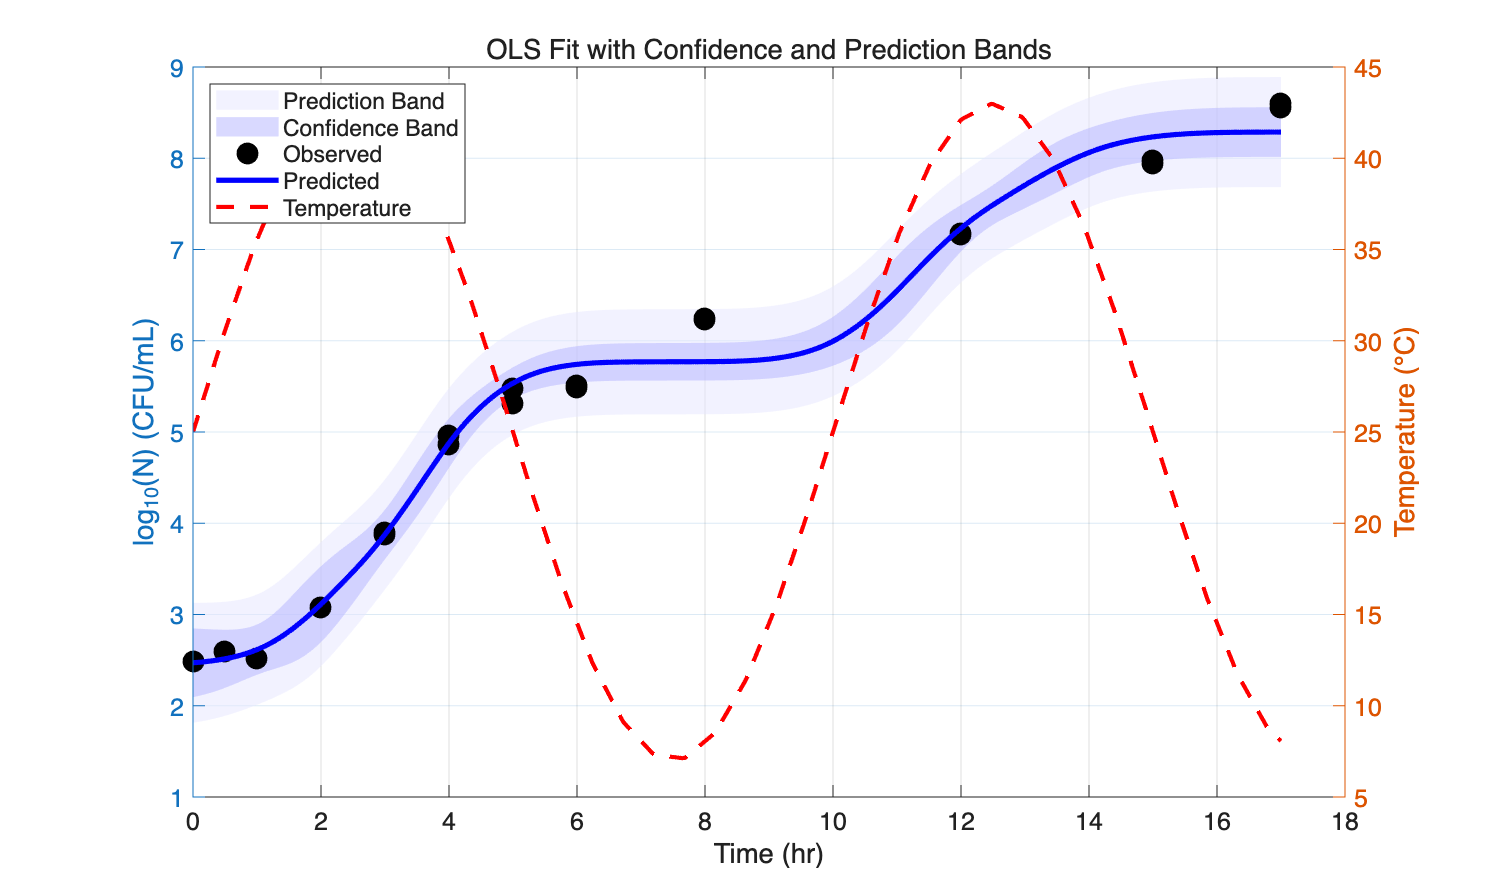
\includegraphics[width=0.72\linewidth]{fig03_fit_CB_PB.png}

{\scriptsize Fig.\,3. OLS fitted curve with 95\% asymptotic confidence band (dark) and prediction band (light).\\Black dots: observed; Blue line: predicted; Red dashed: sinusoidal temperature.}
\end{frame}

% ==================== Slide 9: Residuals ====================
\section{Residual Analysis}
\begin{frame}{Residual Analysis}
\begin{columns}[T]
\begin{column}{0.42\textwidth}
\centering
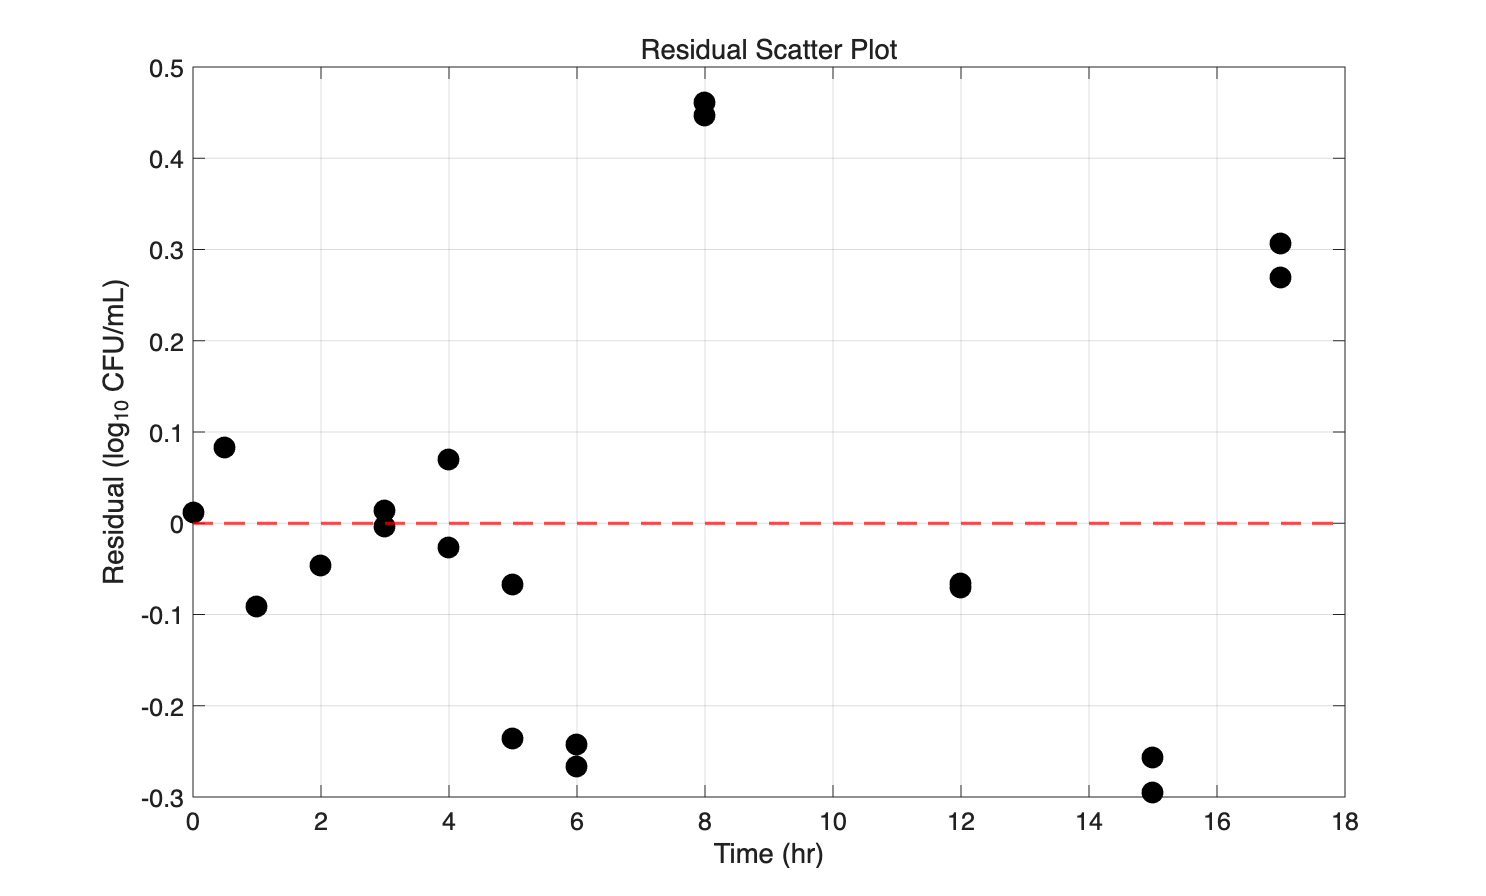
\includegraphics[width=\linewidth]{fig04_residual_scatter.png}

{\scriptsize Fig.\,4. Residuals vs.\ time.\\Random scatter around zero.}
\end{column}
\begin{column}{0.42\textwidth}
\centering
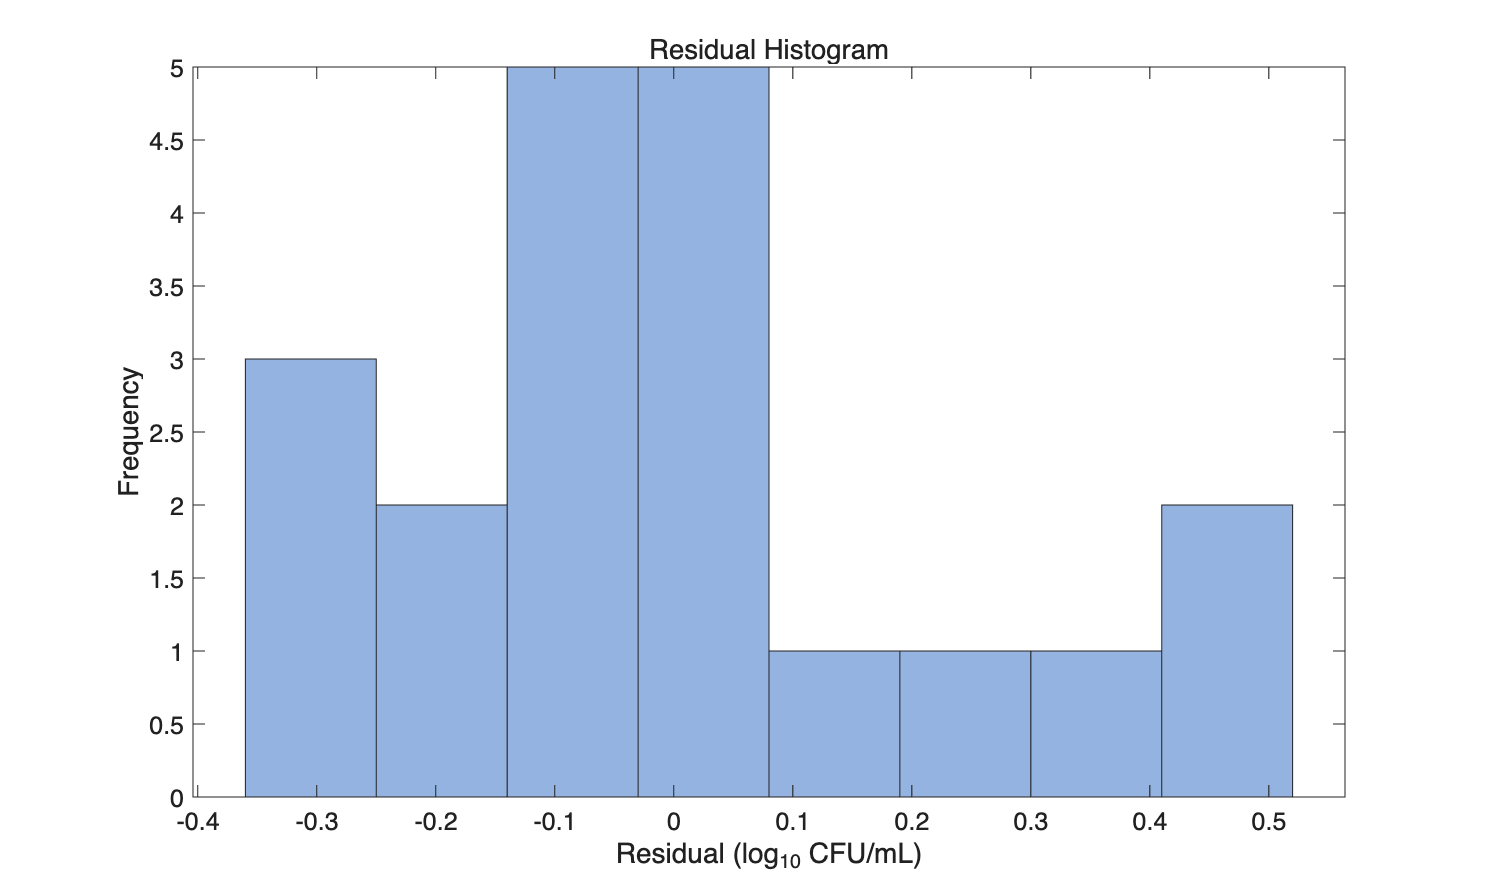
\includegraphics[width=\linewidth]{fig05_residual_histogram.png}

{\scriptsize Fig.\,5. Residual histogram.\\Approximately bell-shaped.}
\end{column}
\end{columns}
\vspace{0.3em}
\centering
{\small
\begin{tabular}{clc}
\toprule
\# & Assumption & Result \\
\midrule
1 & Model is correct      & $\checkmark$ (visual) \\
2 & Errors are random     & DW = 1.3149 \\
3 & Constant variance     & $\checkmark$ (visual) \\
4 & Errors uncorrelated   & See DW \\
5 & Normal distribution   & SW $p$ = 1.0000 ($\checkmark$) \\
\bottomrule
\end{tabular}}

{\scriptsize Table 5. Five standard statistical assumptions.}
\end{frame}

% ==================== Slide 10: Final SSC ====================
\begin{frame}{Final Scaled Sensitivity Coefficients}
\begin{columns}[T]
\begin{column}{0.58\textwidth}
\centering
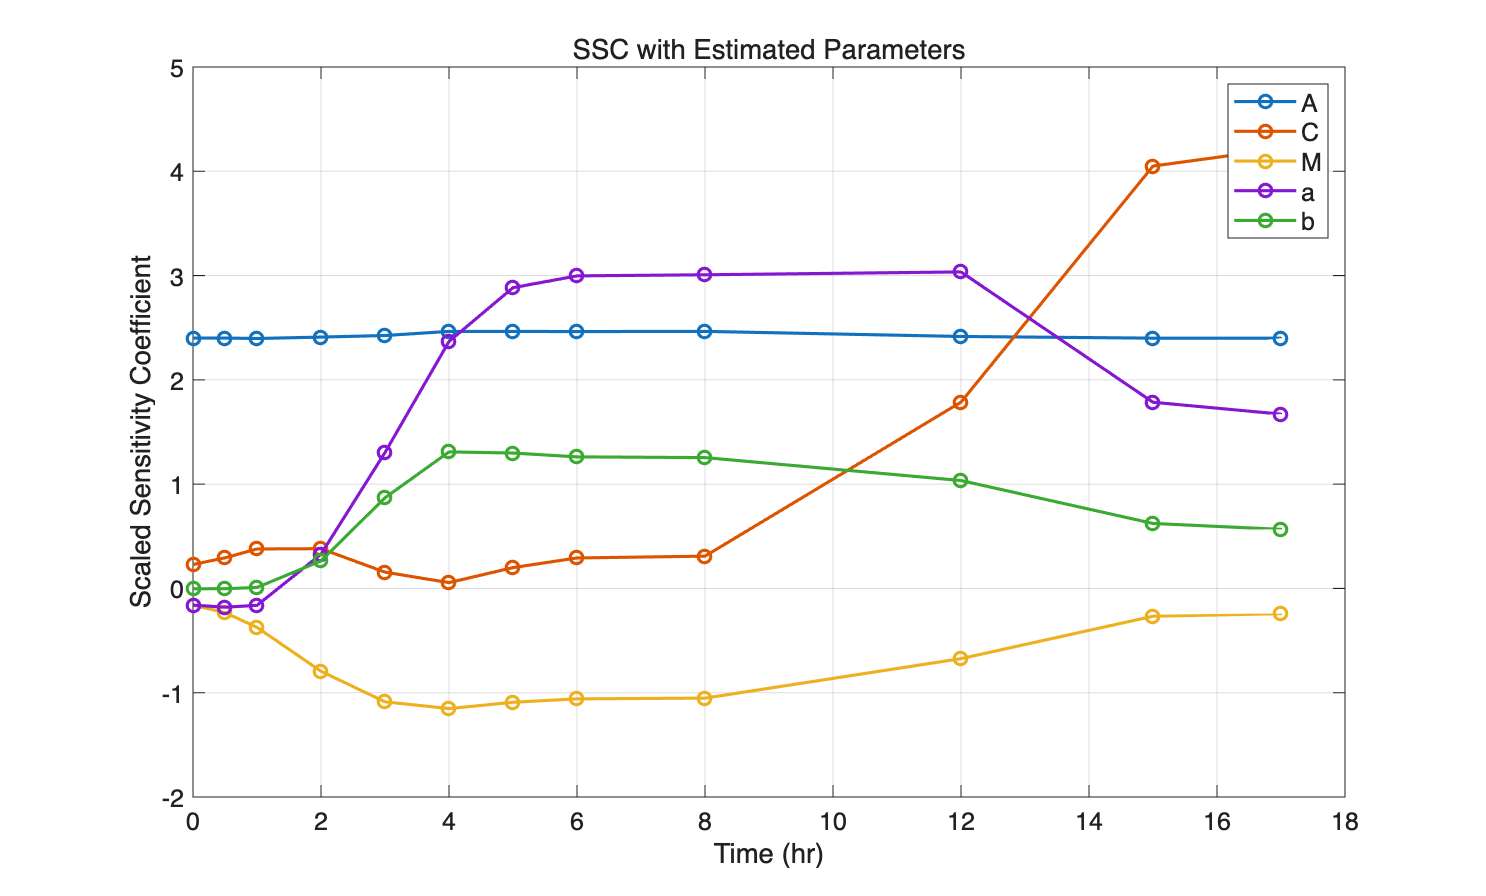
\includegraphics[width=\linewidth]{fig06_ssc_final.png}

{\scriptsize Fig.\,6. SSC recomputed with estimated parameters.\\Patterns consistent with initial SSC.}
\end{column}
\begin{column}{0.38\textwidth}
\centering
{\small
\begin{tabular}{lr}
\toprule
Param & max$|$SSC$|$ \\
\midrule
$A$ & 2.4649 \\
$C$ & 4.2172 \\
$M$ & 1.1521 \\
$a$ & 3.0349 \\
$b$ & 1.3092 \\
\bottomrule
\end{tabular}}

{\scriptsize Table 6. Final SSC magnitudes.}

\vspace{1em}
{\small All parameters identifiable at the OLS solution.}
\end{column}
\end{columns}
\end{frame}

% ==================== Slide 11: OED ====================
\section{Optimal Experimental Design}
\begin{frame}{Optimal Experimental Design}
\begin{columns}[T]
\begin{column}{0.48\textwidth}
\centering
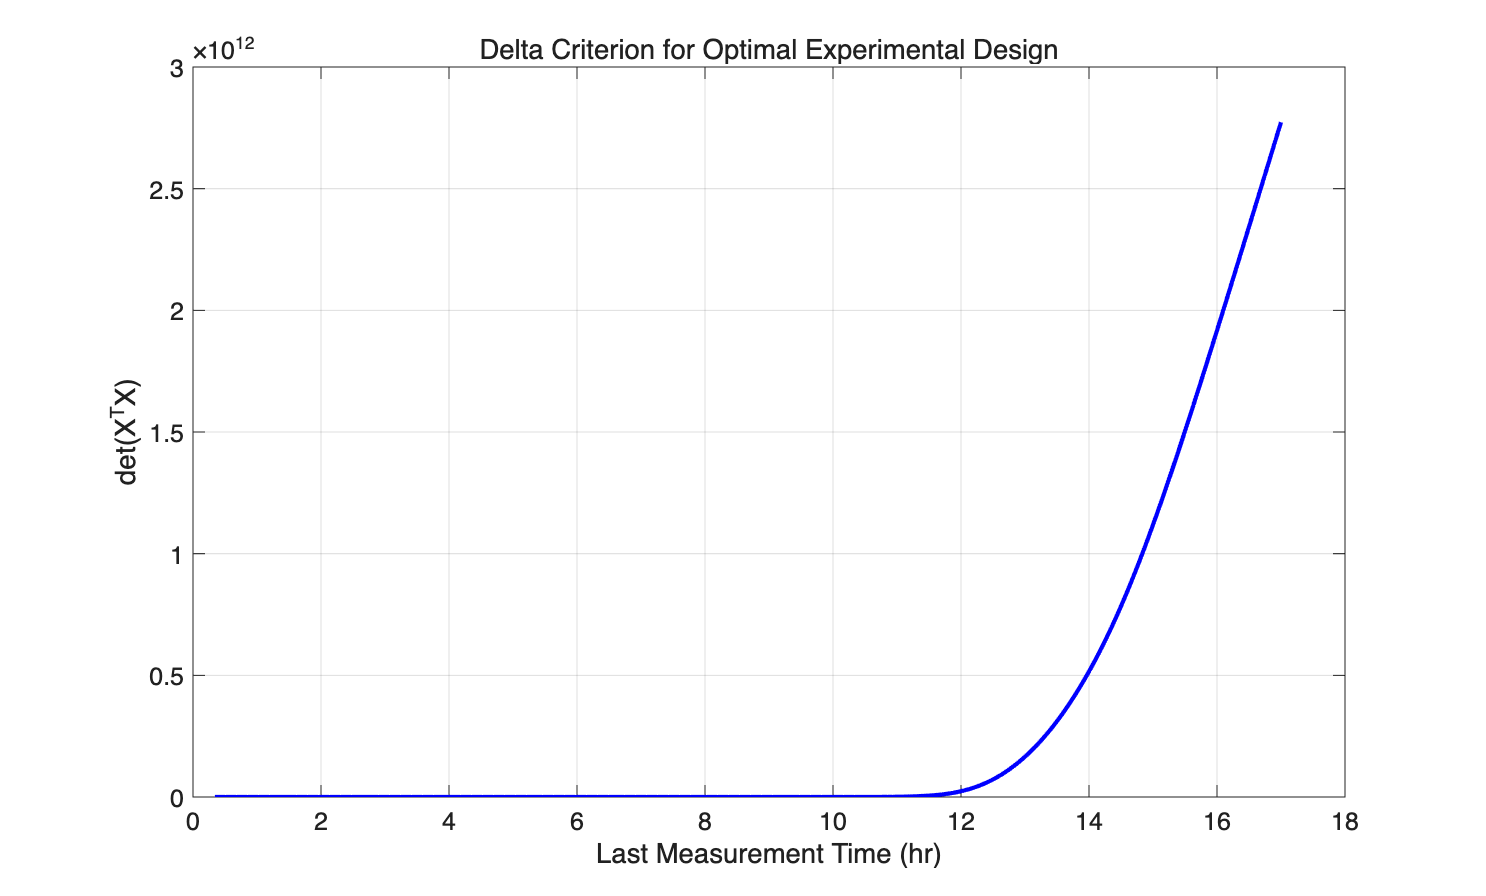
\includegraphics[width=\linewidth]{fig07_delta_criterion.png}

{\scriptsize Fig.\,7. Delta criterion $\det(X^TX)$ vs.\ last measurement time. Increasing trend: more data improves estimation.}
\end{column}
\begin{column}{0.48\textwidth}
\centering
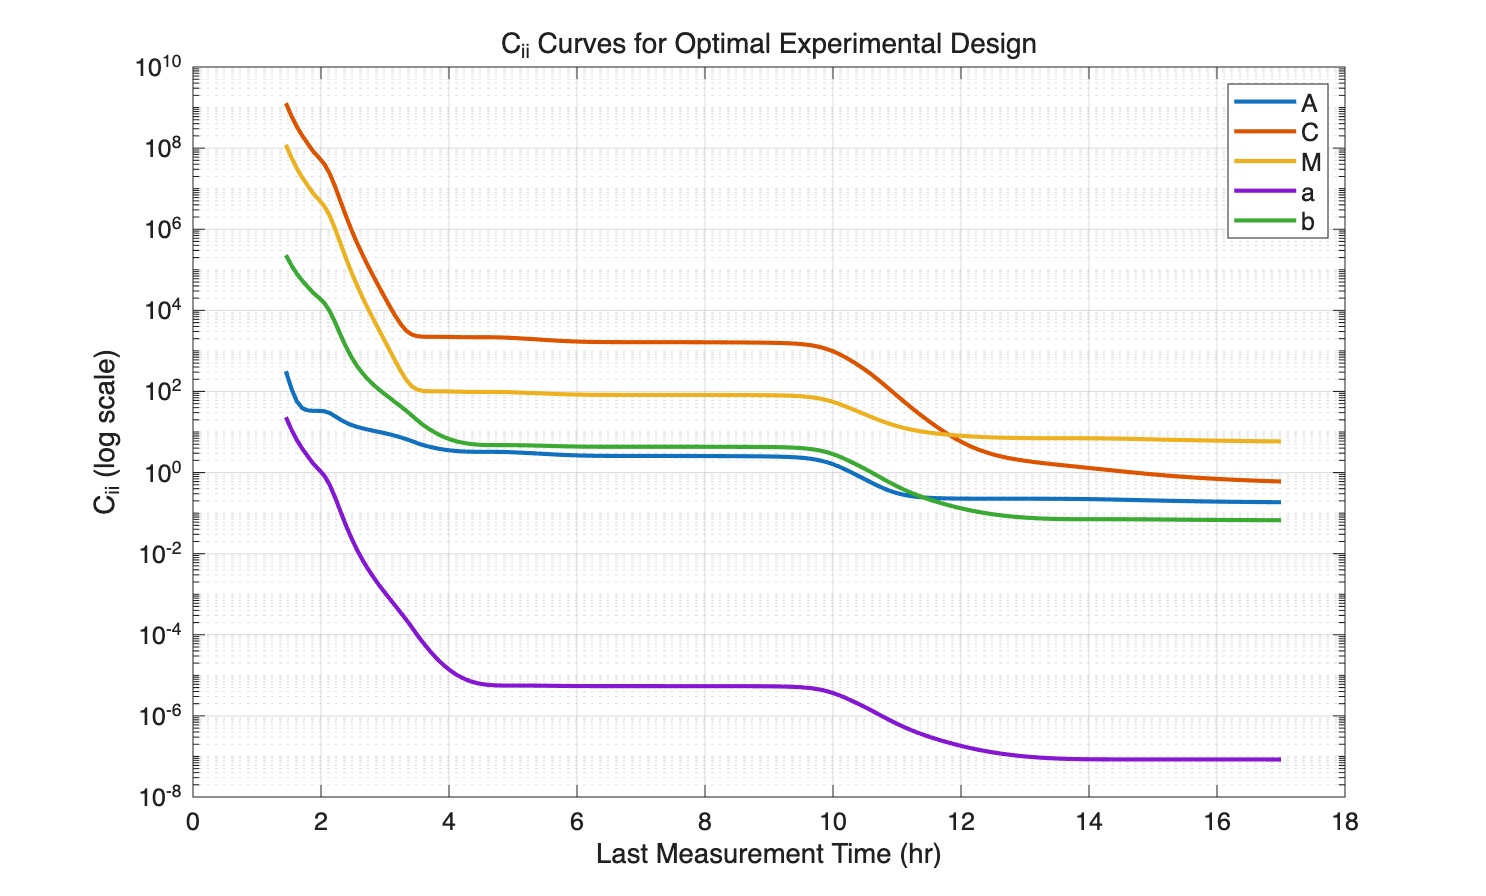
\includegraphics[width=\linewidth]{fig08_Cii_curves.png}

{\scriptsize Fig.\,8. $C_{ii}$ curves (log scale). Decreasing values: parameters become more precise.}
\end{column}
\end{columns}
\vspace{0.3em}
{\small Key measurement window: exponential growth phase ($\sim$2--8\,hr).}
\end{frame}

% ==================== Slide 12: Bootstrap ====================
\section{Bootstrap}
\begin{frame}{Bootstrap Analysis ($N=1000$)}
\begin{columns}[T]
\begin{column}{0.48\textwidth}
\centering
{\footnotesize
\begin{tabular}{lcccc}
\toprule
 & \multicolumn{2}{c}{Bootstrap CI} & \multicolumn{2}{c}{Asymptotic CI} \\
Param & Lower & Upper & Lower & Upper \\
\midrule
$A$ & 1.600 & 2.741 & 1.860 & 2.943 \\
$C$ & 5.761 & 7.819 & 5.407 & 7.353 \\
$M$ & $-$0.624 & 5.388 & $-$0.931 & 6.774 \\
$a$ & 8.81e-4 & 2.11e-3 & 5.75e-4 & 1.70e-3 \\
$b$ & 0.065 & --- & $-$0.203 & 0.727 \\
\bottomrule
\end{tabular}}

{\scriptsize Table 7. Bootstrap vs.\ asymptotic 95\% CI.}

\vspace{0.4em}
{\footnotesize
\begin{tabular}{lc}
\toprule
Band & Avg Width \\
\midrule
Asymptotic CB & 0.5307 \\
Bootstrap CB  & 0.4058 \\
Asymptotic PB & 1.2042 \\
Bootstrap PB  & 1.0720 \\
\bottomrule
\end{tabular}}

{\scriptsize Table 8. Band width comparison.}
\end{column}
\begin{column}{0.48\textwidth}
\centering
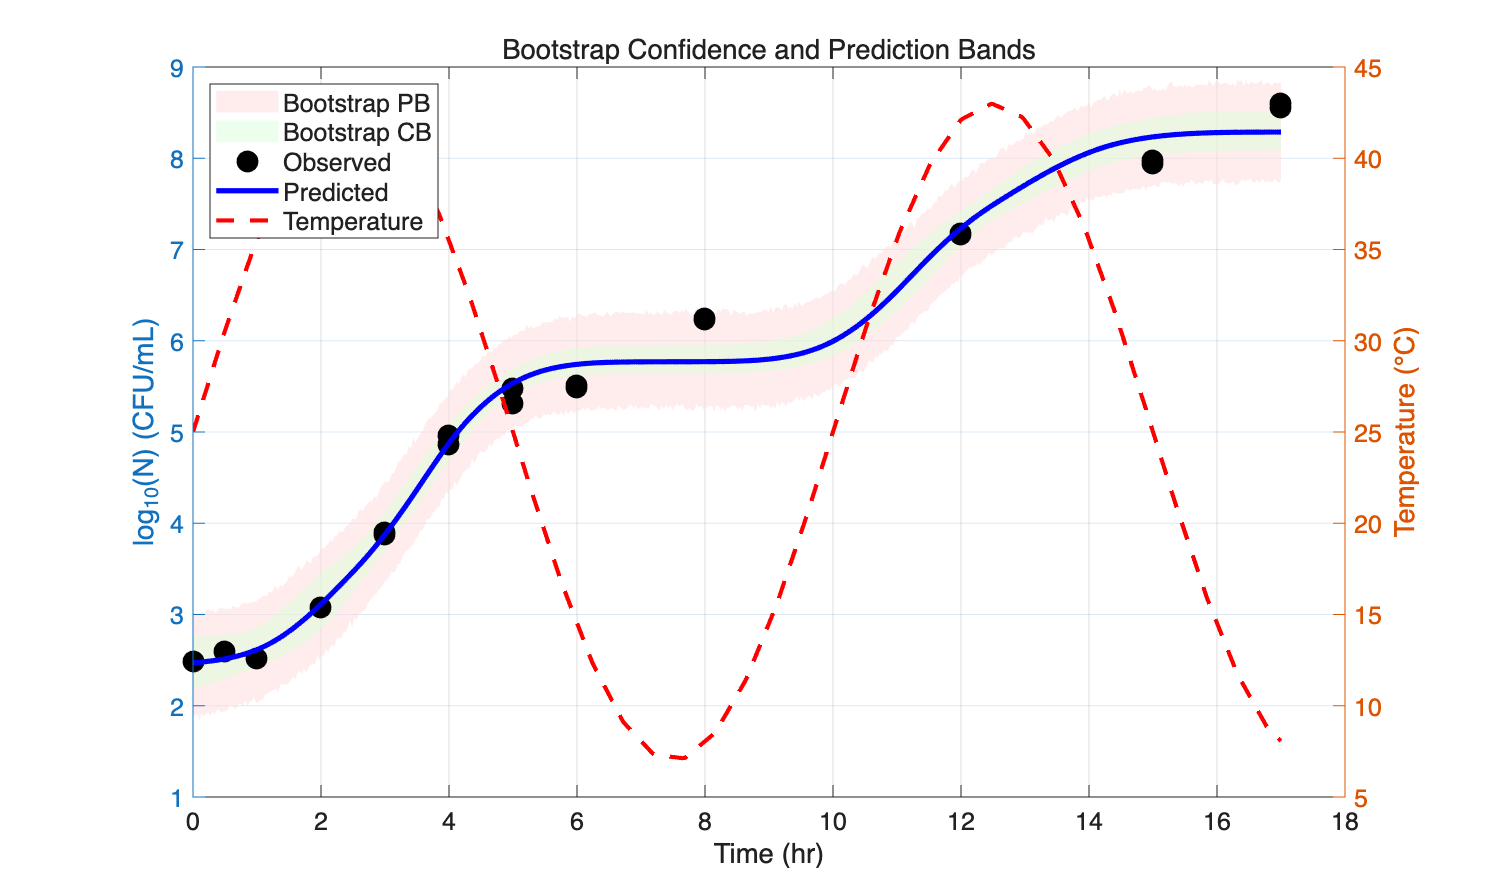
\includegraphics[width=\linewidth]{fig09_bootstrap_CB_PB.png}

{\scriptsize Fig.\,9. Bootstrap CB (green) and PB (pink) from 1000 residual-resampling iterations.}
\end{column}
\end{columns}
\end{frame}

% ==================== Slide 13: Summary ====================
\section{Summary}
\begin{frame}{Summary \& Conclusions}
\begin{itemize}
    \item Dynamic Gompertz model successfully developed for SE growth in egg yolk
    \item 5 parameters estimated, 2 fixed; RMSE = 0.2524 $\log_{10}$ CFU/mL
    \item Pseudo-$R^2$ = 0.9874; all 5 statistical assumptions evaluated
    \item Optimal experimental design: key window at 2--8\,hr
    \item Bootstrap CIs generally consistent with asymptotic CIs
    \item \textbf{Practical significance:} Model predicts SE risk during egg cooling, storage, and distribution --- supports USDA-FSIS 7.2\,$^\circ$C recommendation
\end{itemize}
\end{frame}

% ==================== Slide 14: References ====================
\section{References}
\begin{frame}[allowframebreaks]{References}
\reference
\end{frame}

% ==================== Slide 15: Thank You ====================
\begin{frame}
\centering
\vspace{2cm}
{\Huge Thank You!}
\vspace{1.5cm}

{\Large Questions?}
\end{frame}

\end{document}
